\documentclass[12pt,a4paper]{article}
\usepackage[utf8x]{inputenc}
\usepackage{ucs}
\usepackage{amsmath}
\usepackage{amsfonts}
\usepackage{amssymb}
\usepackage{graphicx}
\usepackage{grffile}
\usepackage{float}
\usepackage{multicol}
\usepackage[portuguese]{babel}
\title{Dinamica}
\author{André Garnier Coutinho}
\setlength{\textwidth}{17cm}
\setlength{\textheight}{24cm}
\addtolength{\topmargin}{-2cm}
\addtolength{\oddsidemargin}{-2cm}
\begin{document}
\begin{center}
\textbf{Escola Politécnica da USP\\
PMR5014 - Controle Não Linear Aplicado a Sist. Mecânicos e Mecatrônicos\\}
\end{center}

\begin{center}
\textbf{Modelagem do pentágono articulado}
\end{center}

\begin{figure}[h!]
	\centering
	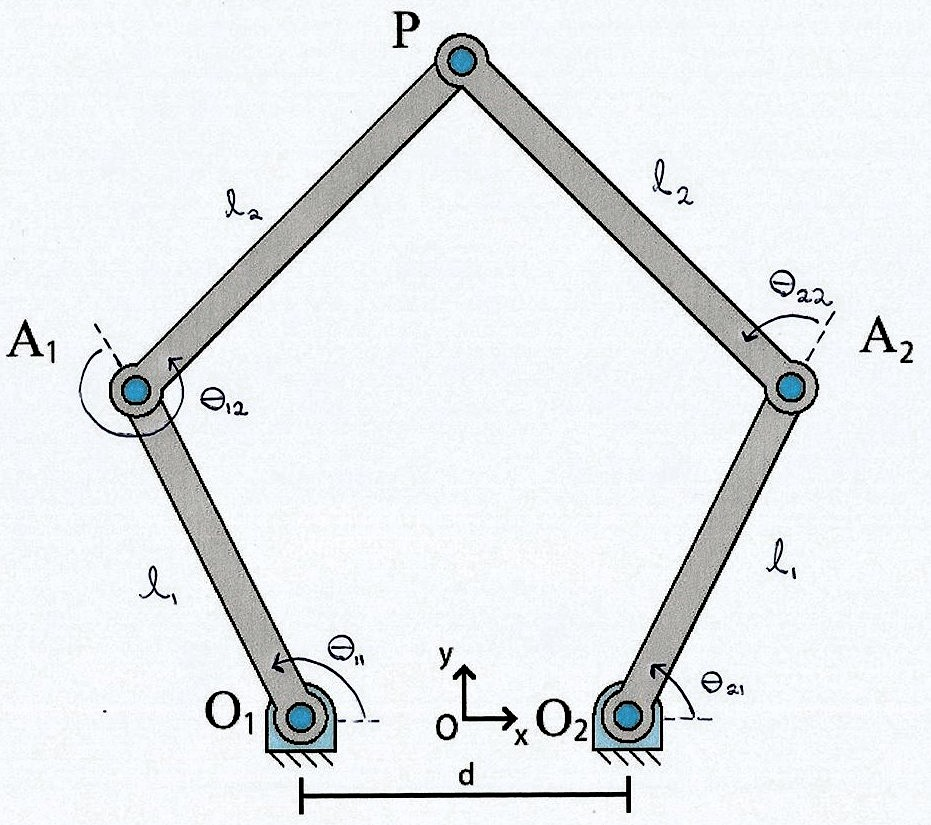
\includegraphics[scale=0.3]{5Rscan.jpg}  
	\caption{Robô 5R}
	\label{fig:figura1}
\end{figure}

\noindent{\bf Análise Cinemática: }

\begin{itemize}
\item[•] Cinemática de Posição \\

	O objetivo da cinemática de posição é encontrar a relação entre as coordenadas $X = (x_p, y_p)$, da plataforma, e as coordenadas $\Theta = (\theta_{11}, \theta_{21})$, dos atuadores.
	Abaixo seguem as coordenadas dos pontos $O_1$, $A_1$, $O_2$, $A_2$, e $P$ em relação ao sistema de coordenadas $O_{xy}$:
	\begin{multicols}{2}
	$ O_1 (-\frac{d}{2}, 0) \\
	A_1 ( -\frac{d}{2} + l_1 c_{11} , l_1 s_{11} ) \\
	P (x_p, y_p) \\
	O_2 (\frac{d}{2}, 0) \\
	A_2 ( \frac{d}{2} + l_1 c_{21} , l_1 s_{21} ) $	
	\end{multicols}
	
	Utilizando as seguintes restrições geométricas, temos:
	
	\begin{equation}
		\begin{cases}
		|| P - A_1 ||^2 = l_2^2 \\
		|| P - A_2 ||^2 = l_2^2 \\
		\end{cases}
		\Rightarrow	
		\begin{cases}
		(x_p +\frac{d}{2} - l_1 c_{11})^2 + (y_p - l_1 s_{11})^2 = l_2^2 \\
		(x_p -\frac{d}{2} - l_1 c_{21})^2 + (y_p - l_1 s_{21})^2 = l_2^2 \\
		\end{cases}
	\end{equation}

		\begin{itemize}
		\item[•] Cinemática Inversa \\
	
		Supondo	conhecidas as coordenadas $X$, deve-se encontrar as coordenadas $\Theta$. \\
		Assim, desenvolvendo a primeira equação do sistema de equações $(1)$:
		
		$$ (x_p +\frac{d}{2})^2 -2 (x_p +\frac{d}{2}) l_1 c_{11} + l_1^2 c_{11}^2 + y_p^2 - 2 y_p l_1 s_{11} + l_1^2 s_{11}^2 = l_2^2   $$
		$$ \Rightarrow -2 (x_p +\frac{d}{2}) l_1 c_{11} - 2 y_p l_1 s_{11} +  (x_p +\frac{d}{2})^2 + y_p^2 + l_1^2 - l_2^2 = 0 $$
		\begin{equation}
		\therefore E_1 c_{11} + F_1 s_{11} + G_1 = 0
		\end{equation}
		
		Sendo:
		
		\begin{equation}	
		\begin{cases}
		E_1 = -2 (x_p +\frac{d}{2}) l_1 \\
		F_1 = - 2 y_p l_1 \\
		G_1 = (x_p +\frac{d}{2})^2 + y_p^2 + l_1^2 - l_2^2
		\end{cases}
		\end{equation}
		
		Cuja solução é dada por:
		
		\begin{equation}
		\theta_{11} =
		\begin{cases}
		2\arctan \Big( \frac{-F_1 + \sqrt{E_1^2 + F_1^2 - G_1^2}}{G_1 - E_1} \Big) , & \mbox{se } G_1 \neq E_1 \\
		2\arctan \Big( -\frac{E_1}{F_1} \Big) , & \mbox{se } G_1 = E_1 \\
		\end{cases}
		\end{equation}	
		
		Para a segunda equação do sistema (1), o procedimento é análogo, resultando em:
		
		\begin{equation}
		\theta_{21} =
		\begin{cases}
		2\arctan \Big( \frac{-F_2 - \sqrt{E_2^2 + F_2^2 - G_2^2}}{G_2 - E_2} \Big) , & \mbox{se } G_2 \neq E_2 \\
		2\arctan \Big( -\frac{E_2}{F_2} \Big) , & \mbox{se } G_2 = E_2 \\
		\end{cases}
		\end{equation}	
		
		Sendo:
		
		\begin{equation}	
		\begin{cases}
		E_2 = -2 (x_p -\frac{d}{2}) l_1 \\
		F_2 = - 2 y_p l_1 \\
		G_2 = (x_p -\frac{d}{2})^2 + y_p^2 + l_1^2 - l_2^2
		\end{cases}
		\end{equation}
					
		

		
		
	    \item[•] Cinemática Direta \\
	
		Supondo	conhecidas as coordenadas $\Theta$, deve-se encontrar as coordenadas $X$. \\
		Podemos reescrever (1) da seguinte forma:
	
		$$
		\begin{cases}
		(x_p - x_{c1})^2 + (y_p - y_{c1})^2 = r^2 \\
		(x_p - x_{c2})^2 + (y_p - y_{c2})^2 = r^2 \\
		\end{cases}
		$$
	
		Sendo:
	
		\begin{equation}
		\begin{cases}
		x_{c1} = -\frac{d}{2} + l_1 c_{11}\\
		x_{c2} =  \frac{d}{2} + l_1 c_{21} \\
		y_{c1} =  l_1 s_{11}\\
		y_{c2} =  l_1 s_{21} \\
		r^2 = l_2^2
		\end{cases}
		\end{equation}
	
		Sendo assim, podemos enxergar (1) como a intersecção de duas circunferências de raio $r$. Desta maneira, pode-se dizer que a solução está contida na reta que passa pelo ponto médio dos centros das circunferências, ortogonal à reta que passa pelos dois centros. \\
	
		Definindo:
	
		\begin{equation}
		\begin{cases}
		x_m = \frac{x_{c1}+x_{c2}}{2} \\
		y_m = \frac{y_{c1}+y_{c2}}{2} \\
		dx = x_{c2} - x_{c1} \\
		dy = y_{c2} - y_{c1} \\	
		\end{cases}
		\end{equation}
	
		A equação vetorial desta reta é dada por:
	
		$$ (x_p, y_p) = (x_m, y_m) + \lambda ( -dy, dx ), \lambda \in \mathbb{R} $$
	
		Ou seja:		
	
		\begin{equation}
		\begin{cases}
		x_p = x_m - \lambda dy \\
		y_p = y_m + \lambda dx
		\end{cases}	
		\end{equation}
	
		Substituindo (9) na primeira equação de (1):
	
		$$ (x_m - \lambda dy  - x_{c1})^2 + (y_m + \lambda dx  - y_{c1})^2 = r^2 $$
		$$ \Big( \frac{dx}{2} - \lambda dy \Big)^2 + \Big( \frac{dy}{2} + \lambda dx \Big)^2 = r^2 $$
		$$ \frac{dx^2}{4} - \lambda dx dy + \lambda^2 dy^2 + \frac{dy^2}{4} + \lambda dx dy + \lambda^2 dx^2 = r^2 $$
		$$ \lambda^2 (dx^2 + dy^2) = r^2 - \frac{dx^2 + dy^2}{4} $$
		$$ \therefore \lambda = \pm \sqrt{ \frac{r^2}{dx^2 + dy^2} - \frac{1}{4} } $$
	
		Sendo assim, para montagem do mecanismo conforme a Figura 1, obtemos:
	
		\begin{equation}
		x_p = x_m - dy \sqrt{ \frac{r^2}{dx^2 + dy^2} - \frac{1}{4} }
		\end{equation}
	
		\begin{equation}
		y_p = y_m + dx \sqrt{ \frac{r^2}{dx^2 + dy^2} - \frac{1}{4} }
		\end{equation} \\
	
	    \item[•] Cinemática dos ângulos intermediários: \\
	
		Supondo que a cinemática direta ou inversa já foi realizada (são conhecidos $X$ e $\Theta$), os ângulos $\theta_{12}$ e $\theta_{22}$ podem se definidos da seguinte maneira:
	
		$$
		\begin{cases}
		\tan ( \theta_{11} + \theta_{12} ) = \frac{y_p - l_1 s_{11}}{x_p +\frac{d}{2} - l_1 c_{11}} \\
		\tan ( \theta_{21} + \theta_{22} ) = \frac{y_p - l_1 s_{21}}{x_p -\frac{d}{2} - l_1 c_{21}} \\
		\end{cases}	
		$$
	
		\begin{equation}
		\therefore
		\begin{cases}
		\theta_{12}  = \arctan( \frac{y_p - l_1 s_{11}}{x_p +\frac{d}{2} - l_1 c_{11}}) - \theta_{11} \\
		\theta_{22}  = \arctan( \frac{y_p - l_1 s_{21}}{x_p -\frac{d}{2} - l_1 c_{21}}) + \pi - \theta_{21}\\
		\end{cases}	
		\end{equation}\\
	
		\end{itemize}
		
	\item[•] Cinemática de velocidades: \\
	
	Com o problema de posição resolvido, podemos facilmente resolver o problema de velocidades, o qual se torna linear. \\
	
	Primeiro, reescrevemos o sistema de equações (1) como um vetor de funções nulas:
	
	\begin{equation}
	\Phi (X, \Theta) = 0
	\end{equation}
	
	Sendo:
	
	\begin{equation}
	\Phi (X, \Theta) =
	\begin{bmatrix}
		(x_p +\frac{d}{2} - l_1 c_{11})^2 + (y_p - l_1 s_{11})^2 - l_2^2 \\
		(x_p -\frac{d}{2} - l_1 c_{21})^2 + (y_p - l_1 s_{21})^2 - l_2^2 \\
	\end{bmatrix}
	\end{equation}	 
	
	Depois, derivamos (13) no tempo, aplicando a regra da cadeia, e dividimos por 2, obtendo:
	
	\begin{equation}
	J_X \dot{X} + J_\Theta \dot{\Theta} = 0
	\end{equation}
	
	Sendo:
	
	\begin{equation}
	J_X = \frac{1}{2} \frac{\partial \Phi}{\partial X} =
	\begin{bmatrix}
	x_p + \frac{d}{2} - l_1 c_{11} & y_p - l_2 s_{11} \\
	x_p - \frac{d}{2} - l_1 c_{21} & y_p - l_2 s_{21} \\ 
	\end{bmatrix}
	\end{equation}
	
	\begin{equation}
	J_\Theta = \frac{1}{2} \frac{\partial \Phi}{\partial \Theta} =
	\begin{bmatrix}
	l_1 [ (x_p + \frac{d}{2} )s_{11} - y_p c_{11} ] & 0 \\
	0 & l_1 [ (x_p - \frac{d}{2} )s_{21} - y_p c_{21} ] \\	
	\end{bmatrix}
	\end{equation}
	
	Desta maneira, conhecendo $\dot{X}$ pode-se determinar $\dot{\Theta}$ ou conhecendo $\dot{\Theta}$ pode-se determinar $\dot{X}$. \\
	
	Além disso, os Jacobianos $J_X$ e $J_\Theta$ podem ser utilizados para encontrar as singularidades cinemáticas do mecanismo. Os pontos singulares terão o determinante de $J_X$ ou de $J_\Theta$ nulo.
	
	\item[•] Cinemática de acelerações: \\
	
	Derivando (15) no tempo, obtemos:
	
	\begin{equation}
	\dot{J}_X \dot{X} + J_X \ddot{X} + \dot{J}_\Theta \dot{\Theta} + J_\Theta \ddot{\Theta} = 0
	\end{equation}
	
	Sendo:
	
	\begin{equation}
	\dot{J}_X =
	\begin{bmatrix}
	\dot{x}_p + l_1 s_{11} \dot{\theta}_{11} & \dot{y}_p - l_1 c_{11} \dot{\theta}_{11} \\
	\dot{x}_p + l_1 s_{21} \dot{\theta}_{21} & \dot{y}_p - l_1 c_{21} \dot{\theta}_{21} \\
	\end{bmatrix}
	\end{equation}
	
	\begin{equation}
	\dot{J}_\Theta =
	\begin{bmatrix}
	l_1 [ ((x_p + \frac{d}{2}) \dot{\theta}_{11} - \dot{y}_p)c_{11} + (\dot{x}_p + y_p \dot{\theta}_{11})s_{11} ] & 0 \\
	0 & l_1 [ ((x_p - \frac{d}{2}) \dot{\theta}_{21} - \dot{y}_p)c_{21} + (\dot{x}_p + y_p \dot{\theta}_{21})s_{21} ]
	\end{bmatrix}
	\end{equation}
	
	Como as coordenadas dos atuadores ($\Theta$) e da plataforma ($X$) e suas respectivas derivadas temporais já foram determinadas anteriormente, conhencendo $\ddot{X}$ pode-se determinar $\ddot{\Theta}$ ou conhencendo $\ddot{\Theta}$ pode-se determinar $\ddot{X}$. 

\end{itemize}

\noindent{\bf Modelo Dinâmico: } \\

Para encontrar as equações diferenciais de movimento do mecanismo, utilizaremos a técnica de acoplamento de sub-sistemas e as metodologia de Gibss-Appel extendida (utilizando coordenadas generalizadas e velocidades generalizadas redundantes), ambas desenvolvidas no trabalho de Renato Orsino. \\

Primeiro dividimos nosso sistema em 3 sub-sistemas mais simples: 2 mecanismos seriais planos do tipo \underline{R}R e um ponto com massa concetrada livre no espaço. Encontramos o modelo dinâmico de cada um separadamente, e depois utilizamos a técnica de acoplamento de sub-sistemas. \\

Para modelar os sub-sistemas seriais, faremos algumas definições importantes:

\begin{itemize}
\item[•]$q^{\#}$: vetor de $n$ coordenadas generalizadas independentes
\item[•]$q^o$: vetor de $m_q$ coordenadas generalizadas redundandes
\item[•]$q$: vetor contendo todas as coordenadas generalizadas. Usualmente $q = \begin{bmatrix} q^{\#} \\q^o \end{bmatrix} $
\item[•]$\phi(q)$: vetor de tamanho $m_q$ dos vínculos de posição, de modo que conhecendo $q^{\#}$ seja possível determinar $q^o$ resolvendo $\phi(q) = 0$
\item[•]$p^{\#}$: vetor de $n$ velocidades generalizadas independentes
\item[•]$p^o$: vetor de $m_p$ velocidades generalizadas redundandes
\item[•]$p$: vetor contendo todas as velocidades generalizadas. Usualmente $p = \begin{bmatrix} p^{\#} \\p^o \end{bmatrix} $
\item[•]$ \Psi(q) = \frac{\partial P^{\#}}{\partial \dot{q}^{\#}}$: Transformação linear inversível que relaciona $ \dot{q}^{\#}$ com $p^{\#}$, ou seja: $ p^{\#} = P^{\#} (q,\dot{q}^{\#}) = \Psi(q) \dot{q}^{\#} $.
\item[•]$ \Gamma(q) = \frac{\partial \dot{Q}}{\partial p}$: Transformação linear que relaciona $p$ com $\dot{q}$, ou seja: $ \dot{q} = \dot{Q} (q,p) = \Gamma(q) p $.
\item[•]$\Lambda(q,p)$: vetor de tamanho $m_q$ dos vínculos de velocidades, de modo que conhecendo $q$ e $p^{\#}$ seja possível determinar $p^o$ resolvendo $\Lambda(q,p) = 0$
\item[•] $\mathbb{C}(q)$: matriz dos vínculos cinemáticos, obtida através $\Lambda(q,p)$. É qualquer matriz que seja complemento ortogonal (nullspace) transposto de $\frac{\partial \Lambda}{\partial p}$. Uma possibilidade conveniente é definir $\mathbb{C}$ tal que $p = \mathbb{C}(q) p^{\#}$.
\end{itemize}

Na dinâmica de sistemas mecânicos multi-corpos, é muito vantajosa a utilização de coordenadas/velocidades generalizadas redundantes, pois a utilização destas diminui a complexidade da utilização dos métodos de dedução das equações de movimento (como Lagrange, Kane e Gibbs-Appell) e em contrapartida torna necessário definir $\phi(q)$, $\Lambda(q,p)$, $\Psi(q)$, $\Gamma(q)$ e  $\mathbb{C}(q)$. \\

Nos métodos citados, é necessário o cálculo das velocidades absolutas dos centros de massa $\vec{v}_{G_i}$ e das velocidades angulares absolutas $\vec{\omega}_i$ de todos os corpos rígidos do sistema, em função de $p$ e $q$. Sendo assim, é conveniente definir o vetor de velocidades generalizadas $p$ como sendo todas as componentes dos $\vec{v}_{G_i}$ e dos $\vec{\omega}_i$, em alguma ordem conveniente. Fazendo isso, tornamos a apliação dos métodos extremamente simples, deixando praticamente toda a complexidade do problema no cálculo de $\phi(q)$, $\Lambda(q,p)$, $\Psi(q)$, $\Gamma(q)$ e  $\mathbb{C}(q)$. \\

\begin{itemize}

\item[•] Modelo do mecanismo \underline{R}\underline{R}

\begin{figure}[h!]
	\centering
	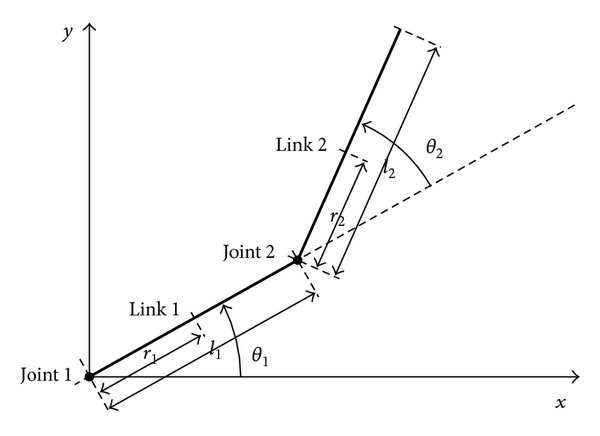
\includegraphics[scale=1.5]{RR.jpg}  
	\caption{Robô \underline{R}\underline{R}}
	\label{fig:figura2}
\end{figure}

	\begin{itemize}
	\item[i)] Primeiro definimos $n + m_q$ coordenadas  $q$. Estas podem ser subdivididas em $n$ coordenadas independentes $q^{\#}$ e $m_q$ 	coordenadas redudantes $q^o$.
	
	$$
	q = \begin{bmatrix}
	q^{\#} \\
	q^o
	\end{bmatrix}
	$$

	No caso do mecanismo $\underline{R}\underline{R}$, temos:

	\begin{equation}
	q^{\#} = \begin{bmatrix}
	\theta_1 & \theta_2
	\end{bmatrix}^T \\
	\end{equation}
	
	\begin{equation}
	q^o = \begin{bmatrix}
	x_1 & y_1 & x_2 & y_2
	\end{bmatrix}^T
	\end{equation}

	Com $n = 2$ e $m_q = 4$. Neste caso, as componentes de $q^o$ são as coordenadas dos centros de massa das barras, escritas no referencial 	inercial $O_{xy}$. \\
	
	\item[ii)] Depois definimos os vetores de velocidades absolutas:
	
	$$ \nu =
	\begin{bmatrix}
	\nu_\omega \\
	\nu_v
	\end{bmatrix}
	$$
	
	\begin{equation}
	\nu_\omega = \begin{bmatrix}
	\omega_{z1} & \omega_{z2}
	\end{bmatrix}^T
	\end{equation}
	
	\begin{equation}
	\nu_v = \begin{bmatrix}
	v_{x1} & v_{y1} & v_{x2} & v_{y2}
	\end{bmatrix}^T
	\end{equation}
	
	Sendo $\nu_v$ as componentes das velocidades absolutas dos centros de massa das barras, escritas nas bases presas às barras, e $\nu_\omega$ as componentes das velocidades angulares absolutas, escritas nas bases presas às barras. \\
	
	\item[iii)] Definimos $n + m_p$ coordenadas  $p$. Estas podem ser subdivididas em $n$ coordenadas independentes $p^{\#}$ e $m_p$ coordenadas redudantes $p^o$. As coordenadas $p^{\#}$ podem ser subdividas em $n_1$ velocidades angulares $\omega^{\#}$ e $n_2$ velocidades lineares $v^{\#}$. As coordenadas $p^o$ podem ser subdividas em $m_{p1}$ velocidades angulares $\omega^o$ e $m_{p2}$ velocidades lineares $v^o$.
	
	
	\begin{multicols}{3}
	$ p = \begin{bmatrix}
	p^{\#} \\
	p^o
	\end{bmatrix} $

	$ p^{\#} = \begin{bmatrix}
	\omega^{\#} \\
	v^{\#}
	\end{bmatrix} $

	$ p^o = \begin{bmatrix}
	\omega^o \\
	v^o
	\end{bmatrix} $

	\end{multicols}
	
	Como é conveniente que as velocidades generalizadas $p$ sejam velocidades absolutas, escolhemos as componentes de $p$ como sendo as mesmas componentes de $\nu$, respeitando a ordenação indicada acima. \\ 

	No caso do mecanismo $\underline{R}\underline{R}$, temos:

	\begin{equation}
	\omega^{\#} = \begin{bmatrix}
	\omega_{z1} \\
	\omega_{z2}
	\end{bmatrix}
	\end{equation}
	
	\begin{equation}
	v^{\#} = \emptyset
	\end{equation}		
	
	\begin{equation}
	\omega^o = \emptyset
	\end{equation}		
	
	\begin{equation}
	v^o = \begin{bmatrix}
	v_{x1} & v_{y1} & v_{x2} & v_{y2}
	\end{bmatrix}^T
	\end{equation}\\

	Com $n_1 = 2$, $n_2 = 0$, $m_{p1} = 0$, $m_{p2} = 4$ e $m_p = m_{p1} + m_{p2} = 4$. \\
	
		\item[iv)] Realizamos a cinemática de posição para os centros de massa das barras, de modo a relacionar as coordenadas $q^o$ com as coordenadas $q^{\#}$. Para isso, utilizamos matrizes de transformação homogênea.



	$$ [H]_{B_1/B_0} =
	\begin{bmatrix}
	 Rot(\theta_1, z_0) & [\overrightarrow{O_0 O_1}]_{B_0} \\
	 0_{2x1} & 1 \\
	\end{bmatrix}
	=
	\begin{bmatrix}
	 c_1 & -s_1 & 0 \\
	 s_1 & c_1 & 0 \\
	 0 & 0 & 1 \\
	\end{bmatrix} ;
	\begin{bmatrix}
	[\overrightarrow{O_1 G_1}]_{B_1} \\
	1
	\end{bmatrix}
	=
	\begin{bmatrix}
	l_{1g} \\
	0 \\
	1 \\
	\end{bmatrix}
	$$

	$$ [H]_{B_2/B_1} =
	\begin{bmatrix}
	 Rot(\theta_2, z_1) & [\overrightarrow{O_1 O_2}]_{B_1} \\
	 0_{2x1} & 1 \\
	\end{bmatrix}
	=
	\begin{bmatrix}
	 c_2 & -s_2 & l_1 \\
	 s_2 & c_2 & 0 \\
	 0 & 0 & 1 \\
	\end{bmatrix} ;
	\begin{bmatrix}
	[\overrightarrow{O_2 G_2}]_{B_2} \\
	1
	\end{bmatrix}
	=
	\begin{bmatrix}
	l_{2g} \\
	0 \\
	1 \\
	\end{bmatrix}
	$$

	$$
	[H]_{B_2/B_0} = [H]_{B_1/B_0} [H]_{B_2/B_1} =
	\begin{bmatrix}
	c_{1+2} & -s_{1+2} & l_1 c_1 \\
	s_{1+2} & c_{1+2} & l_1 s_1 \\
	0 & 0 & 1 \\
	\end{bmatrix}
	$$


	\begin{equation}
	\therefore \begin{bmatrix}
	x_1 \\
	y_1 \\
	1 \\
	\end{bmatrix}
	=
	[H]_{B_1/B_0}
	\begin{bmatrix}
	[\overrightarrow{O_1 G_1}]_{B_1} \\
	1
	\end{bmatrix}
	=
	\begin{bmatrix}
	 l_{1g} c_1 \\
	 l_{1g} s_1 \\
	 1 \\
	\end{bmatrix}
	\end{equation}

	\begin{equation}
	\begin{bmatrix}
	x_2 \\
	y_2 \\
	1 \\
	\end{bmatrix}
	=
	[H]_{B_2/B_0}
	\begin{bmatrix}
	[\overrightarrow{O_2 G_2}]_{B_2} \\
	1
	\end{bmatrix}
	=
	\begin{bmatrix}
	 l_1 c_1 + l_{2g} c_{1+2} \\
	 l_1 s_1 + l_{2g} s_{1+2} \\
	 1 \\
	\end{bmatrix}
	\end{equation}

	Repare que a partir das matrizes de transformação homogênea encontradas, encontramos também as seguintes matrizes de mudança de base:
	
	\begin{equation}
	R_1 = [I]_{B_1/B_0} =
	\begin{bmatrix}
	 c_1 & -s_1  \\
	 s_1 & c_1  \\
	\end{bmatrix}
	\end{equation}
	
	\begin{equation}
	R_2 = [I]_{B_2/B_0} =
	\begin{bmatrix}
	 c_{1+2} & -s_{1+2}  \\
	 s_{1+2} & c_{1+2}  \\
	\end{bmatrix}
	\end{equation}		

	Com a cinemática de posição, conseguimos obter $m_q = 4$ equações vínculares de posição. Sendo assim, o vetor dos vínculos de posição é dado por:
	
	
	\begin{equation}
	\phi(q)
	=
	\begin{bmatrix}
	x_1 - l_{1g} c_1 \\
	y_1 - l_{1g} c_2 \\
	x_2 - l_1 c_1 - l_{2g} c_{1+2} \\
	y_2 - l_1 s_1 - l_{2g} s_{1+2} \\
	\end{bmatrix}
	\end{equation}
	
	\item[v)] Utilizamos as matrizes de rotação para calcular as velocidades angulares em função de $q^{\#}$ e $\dot{q}^{\#}$:
	
	\begin{equation}
	[S(\vec{\omega}_1)]_{B_1} = R_1^T \dot{R}_1 =
	\begin{bmatrix}
	0 & -\dot{\theta}_1  \\
	\dot{\theta}_1 & 0  \\
	\end{bmatrix}
	\Rightarrow
	[\vec{\omega}_1]_{B_1} = \dot{\theta}_1 \hat{k}
	\end{equation}
	
	\begin{equation}
	[S(\vec{\omega}_2)]_{B_2} = R_2^T \dot{R}_2 =
	\begin{bmatrix}
	0 & -\dot{\theta}_1 -\dot{\theta}_2 \\
	\dot{\theta}_1 + \dot{\theta}_2 & 0  \\
	\end{bmatrix}
	\Rightarrow
	[\vec{\omega}_2]_{B_2} = (\dot{\theta}_1 + \dot{\theta}_2) \hat{k}
	\end{equation}
	
	\item[vi)] Derivamos as equações de posição ((29) e (30)) para encontrar as velocidades dos centros de massa:
	
	\begin{equation}
	[\vec{v}_1]_{B_0} =
	\begin{bmatrix}
	\dot{x}_1 \\
	\dot{y}_1 \\
	\end{bmatrix}
	=
	\begin{bmatrix}
	- l_{1g} s_1 \dot{\theta}_1 \\
	l_{1g} c_1 \dot{\theta}_1 \\
	\end{bmatrix}
	\end{equation}
	
	\begin{equation}
	[\vec{v}_2]_{B_0} =
	\begin{bmatrix}
	\dot{x}_2 \\
	\dot{y}_2 \\
	\end{bmatrix}
	=
	\begin{bmatrix}
	- l_1 s_1 \dot{\theta}_1 - l_{2g} s_{1+2} ( \dot{\theta}_1 + \dot{\theta}_2)  \\
	l_1 c_1 \dot{\theta}_1 + l_{2g} c_{1+2} ( \dot{\theta}_1 + \dot{\theta}_2)  \\
	\end{bmatrix}
	\end{equation}
	
	\item[vii)] Passamos as velocidades dos centros de massa para as bases pesas nas barras:

	$$ [\vec{v}_1]_{B_1} = [I]_{B_0/B_1} [\vec{v}_1]_{B_0} = R_1^T [\vec{v}_1]_{B_0} $$
	$$ [\vec{v}_2]_{B_2} = [I]_{B_0/B_2} [\vec{v}_2]_{B_0} = R_2^T [\vec{v}_2]_{B_0} $$
	
	Definindo:
	
	
	\begin{equation}
	\mathbf{R} =
	\begin{bmatrix}
	R_1 & 0_{2x2} \\
	0_{2x2} & R_2
	\end{bmatrix}
	\end{equation}
	
	Temos:
	
	\begin{equation}
	\nu_v = \mathbf{R}^T \dot{q}^o
	\end{equation}
	
	
	\begin{equation}
	\therefore
	\begin{bmatrix}
	v_{x1} \\
	v_{y1} \\
	v_{x2} \\
	v_{y2} \\
	\end{bmatrix}
	=
	\begin{bmatrix}
	c_1 & -s_1 & 0 & 0 \\
	s_1 & c_1 & 0 & 0 \\
	0 & 0 & c_{1+2} & -s_{1+2} \\
	0 & 0 & s_{1+2} & c_{1+2} \\
	\end{bmatrix}^T
	\begin{bmatrix}
	\dot{x}_1 \\
	\dot{y}_1 \\	
	\dot{x}_2 \\
	\dot{y}_2 \\	
	\end{bmatrix}
	=
	\begin{bmatrix}
	0 \\
	l_{1g} \dot{\theta}_1 \\
	l_1 s_2 \dot{\theta}_1\\
	(l_1 c_2 + l_{2g} )\dot{\theta}_1 + l_{2g} \dot{\theta}_2 \\
	\end{bmatrix}
	\end{equation}
	
	\item[viii)] Montamos os vetores $p^{\#}$ e $p^o$ em função de $q^{\#}$ e $\dot{q}^{\#}$:

	\begin{equation}
	p^{\#} = 
	\begin{bmatrix}
	\omega_{z1} \\
	\omega_{z2} \\
	\end{bmatrix}
	= P^{\#} (q^{\#}, \dot{q}^{\#} ) =
	\begin{bmatrix}
	\dot{\theta}_1 \\
	\dot{\theta}_1 +\dot{\theta}_2 \\
	\end{bmatrix}
	\end{equation}
	
	\begin{equation}
	p^o = 
	\begin{bmatrix}
	v_{x1} \\
	v_{y1} \\
	v_{x2} \\
	v_{y2} \\
	\end{bmatrix}
	= P^o (q^{\#}, \dot{q}^{\#} ) =
	\begin{bmatrix}
	0 \\
	l_{1g} \dot{\theta}_1 \\
	l_1 s_2 \dot{\theta}_1\\
	(l_1 c_2 + l_{2g} )\dot{\theta}_1 + l_{2g} \dot{\theta}_2 \\
	\end{bmatrix}
	\end{equation}
	
	\item[ix)] Utilizando o fato de que $P^{\#} (q^{\#}, \dot{q}^{\#} ) $ e $P^o (q^{\#}, \dot{q}^{\#} )$ são lineares em $\dot{q}^{\#}$, encontramos as transformações lineares $\Psi(q)$ e $\Upsilon(q)$ e o vetor dos vínculos de velocidades $\Lambda(q,p)$:
	
	\begin{equation}
	p^{\#} = P^{\#} (q^{\#}, \dot{q}^{\#} ) = \frac{\partial P^{\#}}{\partial \dot{q}^{\#}} \dot{q}^{\#} = \Psi \dot{q}^{\#}
	\end{equation}
	
	\begin{equation}
	p^o = P^o (q^{\#}, \dot{q}^{\#} ) = \frac{\partial P^o}{\partial \dot{q}^{\#}} \dot{q}^{\#} = \Upsilon \dot{q}^{\#}
	\end{equation}

	No caso do mecanismo $\underline{R}\underline{R}$, temos:
	
	\begin{equation}
	\Psi = \frac{\partial P^{\#}}{\partial \dot{q}^{\#}} =
	\begin{bmatrix}
	1 & 0  \\
	1 & 1  \\
	\end{bmatrix}
	\end{equation}
	
	\begin{equation}
	\Upsilon = \frac{\partial P^o}{\partial \dot{q}^{\#}} =
	\begin{bmatrix}
	0 & 0 \\
	l_{1g} & 0 \\
	l_1 s_2 & 0 \\
	l_1 c_2 + l_{2g} & l_{2g} 
	\end{bmatrix}
	\end{equation}\\

	Como $p^{\#}$ e $\dot{q}^{\#}$ são independentes e tem o mesmo tamanho:

	$$ \dot{q}^{\#} = \Psi^{-1} p^{\#} $$
	$$ \Rightarrow  p^o = \Upsilon \Psi^{-1} p^{\#} $$
	\begin{equation}
	\therefore \Lambda(q,p) =  \Upsilon \Psi^{-1} p^{\#} - p^o  = 0
	\end{equation}
	
	\item[x)] A partir dos vínculos de velocidades, encontramos a matriz $\mathbb{C}$ dos vínculos cinemáticos:
	
	$$ p^o = \Upsilon \Psi^{-1} p^{\#} \Rightarrow p =
	\begin{bmatrix}
	I_{nxn}\\
	\Upsilon \Psi^{-1}
	\end{bmatrix}
	p^{\#}
	$$
	
	\begin{equation}
	\therefore \mathbb{C} =
	\begin{bmatrix}
	I_{nxn}\\
	\Upsilon \Psi^{-1}
	\end{bmatrix}
	=
	\begin{bmatrix}
	1 & 0 \\
	0 & 1 \\
	0 & 0 \\
	l_{1g} & 0\\
	l_1 s_{2} & 0 \\
	l_1 c_{2} & l_{2g} \\
	\end{bmatrix}
	\end{equation}
	
	\item[xi)] Como (39) e (43) são transformações inversíveis, encontramos a transformação linear $\Gamma(q)$:
	
	\begin{equation}
	\dot{q} =
	\begin{bmatrix}
	\dot{q}^{\#} \\
	\dot{q}^o \\
	\end{bmatrix}
	= \dot{Q}(q,p) =
	\begin{bmatrix}
	\Psi^{-1} (q) p^{\#} \\
	\mathbf{R} (q) \nu_v (p)
	\end{bmatrix}
	=
	\begin{bmatrix}
	\omega_{z1} \\
	\omega_{z2}-\omega_{z1}\\
	v_{x1} c_1 - v_{y1} s_1 \\
	v_{x1} s_1 + v_{y1} c_1 \\
	v_{x2} c_{1+2} - v_{y2} s_{1+2} \\
	v_{x2} s_{1+2} + v_{y2} c_{1+2} \\
	\end{bmatrix}
	\end{equation}
	
	\begin{equation}
	\Gamma(q) = \frac{\partial \dot{Q}}{\partial p} =
	\begin{bmatrix}
	1 & 0 & 0 & 0 & 0 & 0 \\
	-1 & 1 & 0 & 0 & 0 & 0 \\
	0 & 0 & c_1 & -s_1 & 0 & 0 \\
	0 & 0 & s_1 & c_1 & 0 & 0 \\
	0 & 0 & 0 & 0 & c_{1+2} & -s_{1+2} \\
	0 & 0 & 0 & 0 & s_{1+2} & c_{1+2} \\
	\end{bmatrix}
	\end{equation}

	\item[xii)] Aplicamos o métodos de Gibbs-Appel extendido: \\
	
	O método de Gibbs-Appell apresenta certa simularidade com o método de Lagrange, pois utiliza derivadas de uma função energia para encontrar a equações de movimento do sistema. Porém, a função energia utilizada não é a energia cinética, mas sim a energia de acelerações. A energia de acelerações para um corpo rígido é dada pela seguinte expressão:

	$$ \mathcal{S} = \frac{1}{2} m ( a_G \cdot a_G ) + \frac{1}{2}( \dot{\omega} \cdot \mathbb{I} \dot{\omega} + 2 \dot{\omega} (\omega \wedge 	\mathbb{I} \omega )  )  $$
 
	Sendo $m$ a massa do corpo rígido, $\mathbb{I}$ seu tensor de inércia, $a_G$ o vetor aceleração absoluta de seu centro de massa e $\omega$ o vetor velocidade angular absoluta.  \\

	O modelo dinâmico utilizando o método de Gibbs-Appel extendido, é dado pela seguinte expressão:
	
	\begin{equation}
	\mathbb{C}(q)^T ( \mathbb{M}(q) \dot{p} + \mathbb{V}(q,p) + \mathbb{G}(q)) = (\Psi^T)^{-1} f_{\dot{q}^{\#}} 
	\end{equation}
	
	Com:
	
	\begin{equation}
	\mathbb{M}(q) = \frac{\partial^2 \mathcal{S}}{\partial \dot{p}^2}
	\end{equation}
	
	\begin{equation}
	\mathbb{V}(q,p) =  \frac{\partial \mathcal{S}}{\partial \dot{p}} - \frac{\partial^2 \mathcal{S}}{\partial \dot{p}^2} \dot{p}
	\end{equation}
	
	\begin{equation}
	\mathbb{G}(q) =  \Gamma^T \frac{\partial E_p}{\partial q}
	\end{equation}
	
	Sendo $E_p$ a energia potencial do sistema e $f_{\dot{q}^{\#}}$ os esforços nas direções de $\dot{q}^{\#}$.
	
	No caso do mecanismo $\underline{R}\underline{R}$, temos:
	
	\begin{equation}
	\mathcal{S} = \frac{1}{2} \Big( m_1 ( \dot{v}_{x1}^2 + \dot{v}_{y1}^2 ) + m_2 ( \dot{v}_{x2}^2 + \dot{v}_{y2}^2  ) + J_{z1} \dot{\omega}_{z1}^2 + + J_{z2} \dot{\omega}_{z2}^2 \Big)
	\end{equation}
	
	\begin{equation}
	E_p = m_1 g y_1 + m_2 g y_2
	\end{equation}
	
	Calculando as derivadas:
	
	\begin{equation}
	\mathbb{M}(q) =
	\begin{bmatrix}
	J_{z1} & 0 & 0 & 0 & 0 & 0 \\
	0 & J_{z2} & 0 & 0 & 0 & 0 \\
	0 & 0 & m_1 & 0 & 0 & 0 \\
	0 & 0 & 0 & m_1 & 0 & 0 \\
	0 & 0 & 0 & 0 & m_2 & 0 \\
	0 & 0 & 0 & 0 & 0 & m_2 \\
	\end{bmatrix}
	\end{equation}
	
	\begin{equation}
	\mathbb{V}(q,p) = 0
	\end{equation}
	
	\begin{equation}
	\mathbb{G}(q) =
	\begin{bmatrix}
	0 \\
	0 \\
	m_1 g s_1 \\
	m_1 g c_1 \\
	m_1 g s_{1+2} \\
	m_1 g c_{1+2}\\
	\end{bmatrix}
	\end{equation}
	
	Sendo assim, o modelo dinâmico para o mecanismo \underline{R}\underline{R} é dado por:
	
	\begin{equation}
	\begin{bmatrix}
	1 & 0 \\
	0 & 1 \\
	0 & 0 \\
	l_{1g} & 0\\
	l_1 s_{2} & 0 \\
	l_1 c_{2} & l_{2g} \\
	\end{bmatrix}^T
	\begin{Bmatrix}
		\begin{bmatrix}
		J_{z1} \dot{\omega}_{z11} \\
		J_{z2} \dot{\omega}_{z12} \\
		m_1 \dot{v}_{x11} \\ 
		m_1 \dot{v}_{y11} \\
		m_2 \dot{v}_{x12} \\
		m_2 \dot{v}_{y12} \\
		\end{bmatrix}
		+
		\begin{bmatrix}
		0 \\
		0 \\
		m_1 g s_{1} \\
		m_1 g c_{1} \\
		m_2 g s_{1+2} \\
		m_2 g c_{1+2} \\
		\end{bmatrix}
	\end{Bmatrix}
	=
	\begin{bmatrix}
	1 & 1 \\
	0 & 1 \\
	\end{bmatrix}^{-1}
	\begin{bmatrix}
	\tau_{11} \\
	\tau_{12} \\
	\end{bmatrix}
	\end{equation}
	
	Repare que o modelo não depende das coordenadas $q^o$. Elas foram uteis para a dedução do modelo, mas com o modelo deduzido elas não tem mais utilidade.
	
	
	
	
	\end{itemize}
	
\item[•] Acoplamento de sub-sistemas: \\

Como o modelo do mecanismo \underline{R}\underline{R} já foi deduzido, e sabendo que o modelo de uma massa concetrada livre no espaço é dado por:

\begin{equation}
\begin{cases}
m_p \ddot{x}_p = F_x \\
m_p \ddot{y}_p = F_y \\
\end{cases}
\end{equation}

Obtemos o modelo do pentagono articulado acoplando dois mecanismos \underline{R}\underline{R} e um ponto de massa concentrada livre no espaço. \\

Para fazer isso, seguimos o seguinte procedimento:

\begin{itemize}
	\item[a)] Definimos as coordenadas generalizadas de cada sub-sistema e do sistema acoplado:
	
	\begin{multicols}{3}
	$ q_0 = q_0^{\#} =
	\begin{bmatrix}
	x_p \\
	y_p \\
	\end{bmatrix}	 $ \\
	
	$ q_1 = q_1^{\#} =
	\begin{bmatrix}
	\theta_{11} \\
	\theta_{12} \\
	\end{bmatrix}	 $ \\
	
	$ q_2 = q_2^{\#} =
	\begin{bmatrix}
	\theta_{21} \\
	\theta_{22} \\
	\end{bmatrix}	 $ \\
	\end{multicols}
	
	\begin{multicols}{3}
	$ \mathsf{q} =
	\begin{bmatrix}
	\mathsf{q}^{\#} \\
	\mathsf{q}^o \\
	\end{bmatrix} $ \\
	
	$ \mathsf{q}^{\#} = q_0 $ \\
	
	$ \mathsf{q}^o =
	\begin{bmatrix}
	q_1 \\
	q_2 \\
	\end{bmatrix} $
	\end{multicols}
	
	\item[b)] Definimos as velocidades generalizadas de cada sub-sistema e do sistema acoplado:
	
	\begin{multicols}{3}
	$ p_0 =
	\begin{bmatrix}
	p_0^{\#} \\
	p_0^o \\
	\end{bmatrix}
	$ \\
	
	$ p_0^{\#} =
	\begin{bmatrix}
	v_{px} \\
	v_{py} \\
	\end{bmatrix}
	$ \\
	
	$ p_0^o = \emptyset$
	\end{multicols}
	
	\begin{multicols}{3}
	$ p_1 =
	\begin{bmatrix}
	p_1^{\#} \\
	p_1^o \\
	\end{bmatrix}
	$ \\
	
	$ p_1^{\#} =
	\begin{bmatrix}
	\omega_{z11} \\
	\omega_{z12} \\
	\end{bmatrix}
	$ \\
	
	$ p_1^o = 
	\begin{bmatrix}
	v_{x11} &
	v_{y11} &
	v_{x12} &
	v_{y12} 
	\end{bmatrix}^T		
	$
	\end{multicols}
	
	\begin{multicols}{3}
	$ p_2 =
	\begin{bmatrix}
	p_2^{\#} \\
	p_2^o \\
	\end{bmatrix}
	$ \\
	
	$ p_2^{\#} =
	\begin{bmatrix}
	\omega_{z21} \\
	\omega_{z22} \\
	\end{bmatrix}
	$ \\
	
	$ p_2^o = 
	\begin{bmatrix}
	v_{x21} &
	v_{y21} &
	v_{x22} &
	v_{y22} 
	\end{bmatrix}^T		
	$
	\end{multicols}
	
	\begin{multicols}{3}
	$ \mathsf{p} =
	\begin{bmatrix}
	\mathsf{p}^{\#} \\
	\mathsf{p}^o \\
	\end{bmatrix} $ \\
	
	$ \mathsf{p}^{\#} = p_0^{\#} $ \\
	
	$ \mathsf{p}^o =
	\begin{bmatrix}
	p_0^o \\
	p_1 \\
	p_2 \\
	\end{bmatrix} $
	\end{multicols}
	
	\begin{multicols}{3}
	$ \mathfrak{p} =
	\begin{bmatrix}
	\mathfrak{p}^{\#} \\
	\mathfrak{p}^o \\
	\end{bmatrix} $ \\
	
	$ \mathfrak{p}^{\#} = p_0^{\#} $ \\
	
	$ \mathfrak{p}^o =
	\begin{bmatrix}
	p_1^{\#} \\
	p_2^{\#} \\
	\end{bmatrix} $
	\end{multicols}
	
	\item[c)] Definimos as relações em $q$ e $p$ de cada sub-sistema:
	
	\begin{multicols}{3}
	$ p_0^{\#} = \Psi_0 q_0^{\#} $ \\
	
	$ p_1^{\#} = \Psi_1 q_1^{\#} $ \\
	
	$ p_2^{\#} = \Psi_2 q_2^{\#} $ \\
	\end{multicols}
	
	\begin{multicols}{3}
	$ \Psi_0 =
	\begin{bmatrix}
	1 & 0 \\
	0 & 1 \\
	\end{bmatrix}
	$ \\
	
	$ \Psi_1 =
	\begin{bmatrix}
	1 & 0 \\
	1 & 1 \\
	\end{bmatrix}
	$ \\
	
	$ \Psi_2 =
	\begin{bmatrix}
	1 & 0 \\
	1 & 1 \\
	\end{bmatrix}
	$ \\
	\end{multicols}
	
	\begin{multicols}{3}
	$ p_0 = \mathbb{C}_0 p_0^{\#} $ \\
	
	$ p_1 = \mathbb{C}_1 p_1^{\#} $ \\
	
	$ p_2 = \mathbb{C}_2 p_2^{\#} $ \\
	\end{multicols}
	
	\begin{multicols}{3}
	$ \mathbb{C}_0 =
	\begin{bmatrix}
	1 & 0 \\
	0 & 1 \\
	\end{bmatrix}
	$ \\
	
	$ \mathbb{C}_1 =
	\begin{bmatrix}
	1 & 0 \\
	0 & 1 \\
	0 & 0 \\
	l_{1g} & 0\\
	l_1 s_{12} & 0 \\
	l_1 c_{12} & l_{2g} \\
	\end{bmatrix}
	$ \\
	
	$ \mathbb{C}_2 =
	\begin{bmatrix}
	1 & 0 \\
	0 & 1 \\
	0 & 0 \\
	l_{1g} & 0\\
	l_1 s_{22} & 0 \\
	l_1 c_{22} & l_{2g} \\
	\end{bmatrix}
	$ \\
	\end{multicols}
	
	Repare que:
	
	\begin{equation}
	\begin{bmatrix}
	p_0 \\
	p_1 \\
	p_2 \\
	\end{bmatrix}
	=
	\begin{bmatrix}
	\mathbb{C}_0 & 0 & 0 \\
	0 & \mathbb{C}_1 & 0 \\
	0 & 0 & \mathbb{C}_2 \\
	\end{bmatrix}
	\begin{bmatrix}
	p_0^{\#} \\
	p_1^{\#} \\
	p_2^{\#} \\
	\end{bmatrix}
	\Rightarrow
	\mathsf{p} =
	\begin{bmatrix}
	\mathbb{C}_0 & 0 & 0 \\
	0 & \mathbb{C}_1 & 0 \\
	0 & 0 & \mathbb{C}_2 \\
	\end{bmatrix}
	\mathfrak{p}
	\end{equation}
	
	Nosso objetivo é encontrar uma matriz $\hat{\mathbb{C}}$ tal que:
	
	\begin{equation}
	\mathfrak{p} = \hat{\mathbb{C}} \mathfrak{p}^{\#} = \hat{\mathbb{C}} \mathsf{p}^{\#}
	\end{equation}
	
	Assim teriamos uma relação linear direta entre $\mathsf{p}$ e $\mathsf{p}^{\#}$. \\
	Nomeamos $\hat{\mathbb{C}}$ de matriz de acoplamento dos sub-sistemas. \\
	
	\item[d)] Encontramos $\dim (\mathsf{q}^o)$ equações vinculares de posição: \\	
	
	Para o pentágono articulado, obtemos 4 equações:
	
	\begin{equation}
	\varphi(q_0,q_1,q_2) =
	\begin{bmatrix}
	x_p +\frac{d}{2} - l_1 c_{11} - l_2 c_{11+12} \\
	y_p - l_1 s_{11} - l_2 s_{11+12} \\
	x_p - \frac{d}{2} - l_1 c_{21} - l_2 c_{21+22} \\
	y_p - l_1 s_{21} - l_2 s_{21+22} \\
	\end{bmatrix}
	= 0
	\end{equation}
	
	\item[e)] Derivamos $\varphi(q_0,q_1,q_2) = 0$ no tempo, utilizando a regra da cadeia, para encontrar os vínculos de velocidades:
	
	$$ \frac{d}{dt}\varphi(q_0,q_1,q_2) = \frac{\partial \varphi}{\partial q_0} \dot{q}_0 + \frac{\partial \varphi}{\partial q_1} \dot{q}_1 + \frac{\partial \varphi}{\partial q_2} \dot{q}_2 = $$
	$$\frac{\partial \varphi}{\partial q_0} \Psi_0^{-1} p_0^{\#} + \frac{\partial \varphi}{\partial q_1} \Psi_1^{-1} p_1^{\#} + \frac{\partial \varphi}{\partial q_2} \Psi_2^{-1} p_2^{\#} = 0 $$
	
	\begin{equation}
	\therefore \mathsf{\Lambda}(\mathsf{q}, \mathfrak{p}^{\#}, \mathfrak{p}^o) =  \frac{\partial \varphi}{\partial q_0} \Psi_0^{-1} p_0^{\#} + \frac{\partial \varphi}{\partial q_1} \Psi_1^{-1} p_1^{\#} + \frac{\partial \varphi}{\partial q_2} \Psi_2^{-1} p_2^{\#} = 0 
	\end{equation}
	
	Para o pentágono articulado:
	
	\begin{equation}
	\mathsf{\Lambda}(\mathsf{q}, \mathfrak{p}^{\#}, \mathfrak{p}^o) =
	\begin{bmatrix}
	v_{px} + \omega_{z11} l_1 s_{11}  + \omega_{z12} l_2 s_{11+12}  \\
	v_{py} - \omega_{z11} l_1 c_{11}  - \omega_{z12} l_2 c_{11+12} \\
	v_{px} + \omega_{z21} l_1 s_{21}  + \omega_{z22} l_2 s_{21+22} \\
	v_{py} - \omega_{z21} l_1 c_{21}  - \omega_{z22} l_2 c_{21+22} \\
	\end{bmatrix}
	\end{equation}
	
	\item[f)] Utilizamos a linearidade de $\mathsf{\Lambda}(\mathsf{q}, \mathfrak{p}^{\#}, \mathfrak{p}^o)$ em $\mathfrak{p}^{\#}$ e $\mathfrak{p}^o$ para encontrar a matriz $\mathbb{C}$:
	
	\begin{equation}
	\mathsf{\Lambda}(\mathsf{q}, \mathfrak{p}^{\#}, \mathfrak{p}^o) = \frac{\partial \mathsf{\Lambda}}{\partial \mathfrak{p}^{\#}} \mathfrak{p}^{\#} + \frac{\partial \mathsf{\Lambda}}{\partial \mathfrak{p}^o} \mathfrak{p}^o = 0 
	\end{equation}
	
	\begin{equation}
	\Rightarrow\mathfrak{p}^o = - \frac{\partial \mathsf{\Lambda}}{\partial \mathfrak{p}^o}^{-1} \frac{\partial \mathsf{\Lambda}}{\partial \mathfrak{p}^{\#}} \mathfrak{p}^{\#}
	\end{equation}
	
	\begin{equation}
	\therefore \hat{\mathbb{C}} =
	\begin{bmatrix}
	I_{2x2} \\
	- \frac{\partial \mathsf{\Lambda}}{\partial \mathfrak{p}^o}^{-1} \frac{\partial \mathsf{\Lambda}}{\partial \mathfrak{p}^{\#}}
	\end{bmatrix}
	\end{equation}
	
	Para o pentágono articulado:
	
	\begin{equation}
	\hat{\mathbb{C}} =
	\begin{bmatrix}
	1 & 0 \\
	0 & 1 \\
	\frac{c_{11+12}}{l_1 s_{12}} & \frac{s_{11+12}}{l_1 s_{12}} \\
	-\frac{c_{11}}{l_2 s_{12}} & -\frac{s_{11}}{l_2 s_{12}} \\
	\frac{c_{21+22}}{l_1 s_{22}} & \frac{s_{21+22}}{l_1 s_{22}} \\
	-\frac{c_{21}}{l_2 s_{22}} & -\frac{s_{21}}{l_2 s_{22}} \\
	\end{bmatrix}
	\end{equation}
	
	\item[g)] Modelo final:
	
\end{itemize}

\end{itemize}

\begin{equation}
\begin{bmatrix}
1 & 0 \\
0 & 1 \\
\frac{c_{11+12}}{l_1 s_{12}} & \frac{s_{11+12}}{l_1 s_{12}} \\
-\frac{c_{11}}{l_2 s_{12}} & -\frac{s_{11}}{l_2 s_{12}} \\
\frac{c_{21+22}}{l_1 s_{22}} & \frac{s_{21+22}}{l_1 s_{22}} \\
-\frac{c_{21}}{l_2 s_{22}} & -\frac{s_{21}}{l_2 s_{22}} \\
\end{bmatrix}^T
\begin{bmatrix}
	\begin{bmatrix}
	m_p \dot{v}_{px}  \\
	m_p \dot{v}_{py} \\
	\end{bmatrix}
	+
	\begin{bmatrix}
	0 \\
	m_p g \\
	\end{bmatrix}
	-
	\begin{bmatrix}
	F_x \\
	F_y \\
	\end{bmatrix}	 \\		
	
	\begin{bmatrix}
	1 & 0 \\
	0 & 1 \\
	0 & 0 \\
	l_{1g} & 0\\
	l_1 s_{12} & 0 \\
	l_1 c_{12} & l_{2g} \\
	\end{bmatrix}^T
	\begin{Bmatrix}
		\begin{bmatrix}
		J_{z1} \dot{\omega}_{z11} \\
		J_{z2} \dot{\omega}_{z12} \\
		m_1 \dot{v}_{x11} \\ 
		m_1 \dot{v}_{y11} \\
		m_2 \dot{v}_{x12} \\
		m_2 \dot{v}_{y12} \\
		\end{bmatrix}
		+
		\begin{bmatrix}
		0 \\
		0 \\
		m_1 g s_{11} \\
		m_1 g c_{11} \\
		m_2 g s_{11+12} \\
		m_2 g c_{11+12} \\
		\end{bmatrix}
	\end{Bmatrix}
	-
	\begin{bmatrix}
	1 & 1 \\
	0 & 1 \\
	\end{bmatrix}^{-1}
	\begin{bmatrix}
	\tau_{11} \\
	\tau_{12} \\
	\end{bmatrix}
	 \\	
	\begin{bmatrix}
	1 & 0 \\
	0 & 1 \\
	0 & 0 \\
	l_{1g} & 0\\
	l_1 s_{22} & 0 \\
	l_1 c_{22} & l_{2g} \\
	\end{bmatrix}^T
	\begin{Bmatrix}
		\begin{bmatrix}
		J_{z1} \dot{\omega}_{z21} \\
		J_{z2} \dot{\omega}_{z22} \\
		m_1 \dot{v}_{x21} \\ 
		m_1 \dot{v}_{y21} \\
		m_2 \dot{v}_{x22} \\
		m_2 \dot{v}_{y22} \\
		\end{bmatrix}
				+
		\begin{bmatrix}
		0 \\
		0 \\
		m_1 g s_{21} \\
		m_1 g c_{21} \\
		m_2 g s_{21+22} \\
		m_2 g c_{21+22} \\
		\end{bmatrix}
	\end{Bmatrix}
	-
	\begin{bmatrix}
	1 & 1 \\
	0 & 1 \\
	\end{bmatrix}^{-1}
	\begin{bmatrix}
	\tau_{21} \\
	\tau_{22} \\
	\end{bmatrix}
	 \\
\end{bmatrix}
=
\begin{bmatrix}
0 \\
0
\end{bmatrix}
\end{equation}	

Que pode ser reescrito como:

\begin{equation}
\left(
\begin{array}{cc}
 1 & 0 \\
 0 & 1 \\
 \frac{c_{11+12} }{l_1 s_{12}} & \frac{s_{11+12}}{l_1 s_{12}} \\
 -\frac{c_{11}}{l_2 s_{12}} & -\frac{s_{11}}{l_2 s_{12} } \\
 0 & 0 \\
 \frac{l_{\text{1g}} c_{11+12}}{l_1 s_{12}} & \frac{l_{\text{1g}} s_{11+12} }{l_1 s_{12}} \\
 c_{11+12} & s_{11+12} \\
  \frac{l_2 c_{12} c_{11+12} - l_{\text{2g}} c_{11}}{l_2 s_{12}} &  \frac{l_2 c_{12} s_{11+12} - l_{\text{2g}} s_{11} }{l_2 s_{12}}  \\
 \frac{c_{21+22}}{l_1 s_{22}} & \frac{s_{21+22}}{l_1 s_{22}} \\
 -\frac{c_{21} }{l_2 s_{22}} & -\frac{s_{21}}{l_2 s_{22}} \\
 0 & 0 \\
 \frac{l_{\text{1g}} c_{21+22}}{l_1 s_{22}} & \frac{l_{\text{1g}} s_{21+22} }{l_1 s_{22}} \\
 c_{21+22} & s_{21+22} \\
  \frac{l_2 c_{22} c_{21+22} - l_{\text{2g}} c_{21}}{l_2 s_{22}} & \frac{l_2 c_{22} s_{21+22} - l_{\text{2g}} s_{21}}{l_2 s_{22}}  \\
\end{array}
\right)^T
\begin{Bmatrix}
	\begin{bmatrix}
	m_p \dot{v}_{px}  \\
	m_p \dot{v}_{py} \\
	J_{z1} \dot{\omega}_{z11} \\
	J_{z2} \dot{\omega}_{z12} \\
	m_1 \dot{v}_{x11} \\ 
	m_1 \dot{v}_{y11} \\
	m_2 \dot{v}_{x12} \\
	m_2 \dot{v}_{y12} \\
	J_{z1} \dot{\omega}_{z21} \\
	J_{z2} \dot{\omega}_{z22} \\
	m_1 \dot{v}_{x21} \\ 
	m_1 \dot{v}_{y21} \\
	m_2 \dot{v}_{x22} \\
	m_2 \dot{v}_{y22} \\
	\end{bmatrix}
	+
	\begin{bmatrix}
	0 \\
	m_p g \\
	0 \\
	0 \\
	m_1 g s_{11} \\
	m_1 g c_{11} \\
	m_2 g s_{11+12} \\
	m_2 g c_{11+12} \\
	0 \\
	0 \\
	m_1 g s_{21} \\
	m_1 g c_{21} \\
	m_2 g s_{21+22} \\
	m_2 g c_{21+22} \\
	\end{bmatrix}
\end{Bmatrix}
=
\begin{bmatrix}
\frac{c_{11+12}}{l_1 s_{12}} & \frac{c_{21+22}}{l_1 s_{22}}\\
\frac{s_{11+12}}{l_1 s_{12}} & \frac{s_{21+22}}{l_1 s_{22}}\\
\end{bmatrix}
\begin{bmatrix}
\tau_{11} \\
\tau_{21} \\
\end{bmatrix}
\end{equation}

Supondo $F_x = F_y = \tau_{12} = \tau_{22} = 0$

$$\mathbb{a}$$


\end{document}
